\documentclass{beamer}

\usepackage{pgfplots}
\usepackage{appendixnumberbeamer}
\usepackage{multirow}

\usetheme{metropolis}

% Metro
%\definecolor{custom_one}{HTML}{d11141}
%\definecolor{custom_two}{HTML}{00b159}
%\definecolor{custom_three}{HTML}{00aedb}
%\definecolor{custom_four}{HTML}{f37735}
%\definecolor{custom_five}{HTML}{ffc425}

%Eeries
%\definecolor{custom_one}{HTML}{11151c}
%\definecolor{custom_two}{HTML}{212d40}
%\definecolor{custom_three}{HTML}{364156}
%\definecolor{custom_four}{HTML}{7d4e57}
%\definecolor{custom_five}{HTML}{d66853}

%Catalogue
\definecolor{custom_one}{HTML}{edc951}
\definecolor{custom_two}{HTML}{eb6841}
\definecolor{custom_three}{HTML}{cc2a36}
\definecolor{custom_four}{HTML}{4f372d}
\definecolor{custom_five}{HTML}{00a0b0}

\title{Classification of Cardiovascular Age by Single-Particle Tracking Method of Deep Learning}
\date{\today}
\author{Maximilian Pfundstein}
\institute{Linköpings University}

\setbeamertemplate{frame footer}{Master Thesis (732A64)}

\begin{document}
    \maketitle
    
    \begin{frame}{Table of contents}
      \setbeamertemplate{section in toc}[sections numbered]
      \tableofcontents%[hideallsubsections]
    \end{frame}
    
    \section{Introduction}
    \begin{frame}{Introduction | ECG and HRV}
        \begin{itemize}
            \item Electrocardiography (ECG) measures the electrical potential of the heart
            \item Heart Rate Variability (HRV) is the variation in time
        \end{itemize}
    \end{frame}
    
    \begin{frame}{Introduction | QRS Complex}
        \begin{figure}[hbt]
        	\center
        	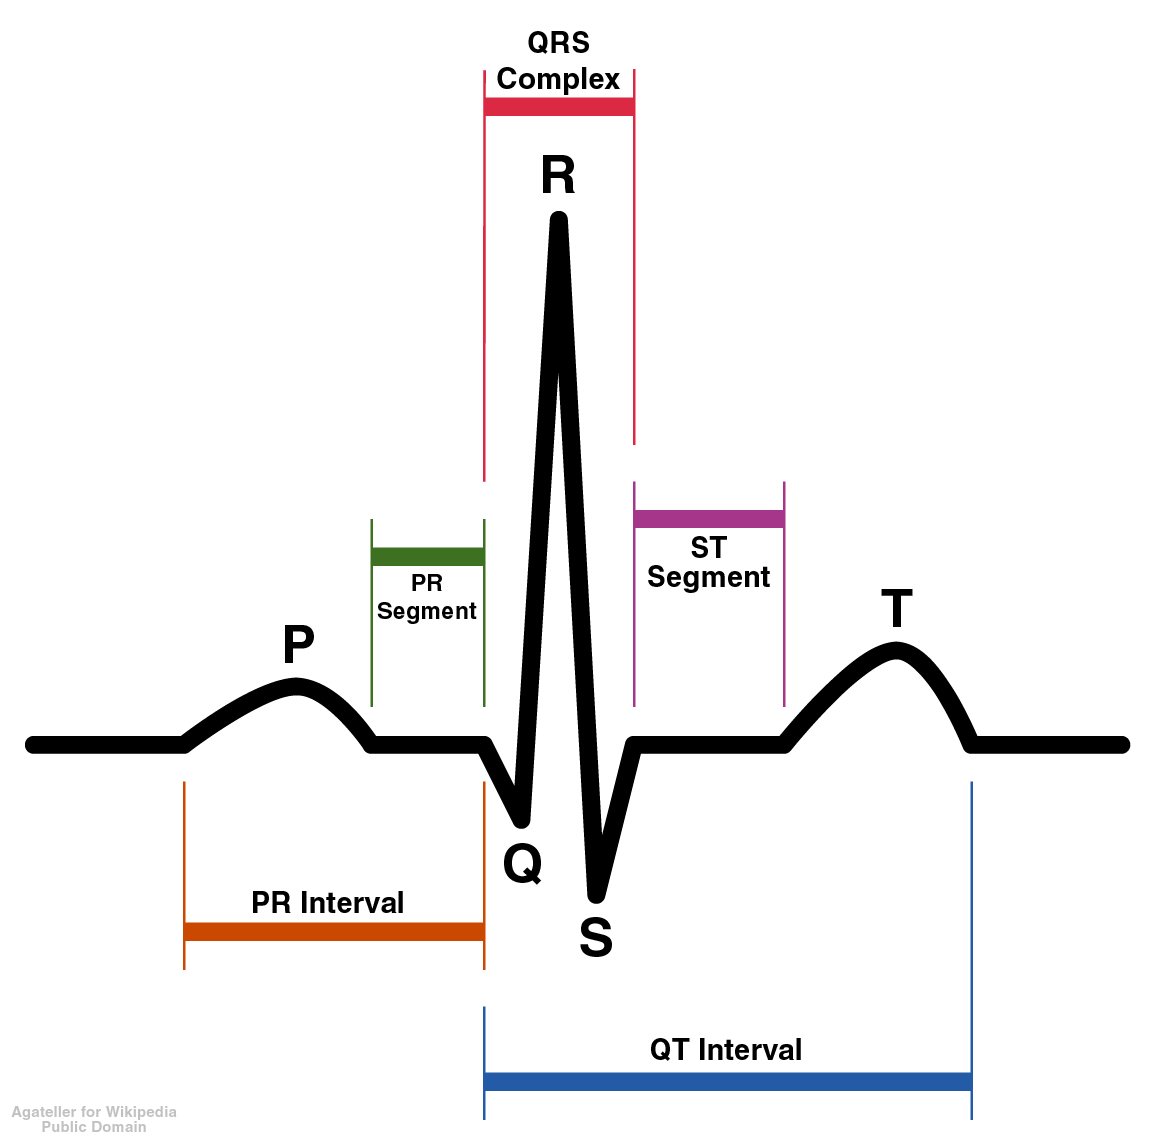
\includegraphics[width=0.55\textwidth]{img/QRS.png}
        	%\caption{ECG in sine rhythm.}
 
        	\label{fig:qrs}
        \end{figure}
        \textbf{Source:} \url{https://en.wikipedia.org/wiki/File:SinusRhythmLabels.png}
    \end{frame}
    
    \begin{frame}{Introduction | RR Interval}
        \begin{figure}[hbt]
        	\center
        	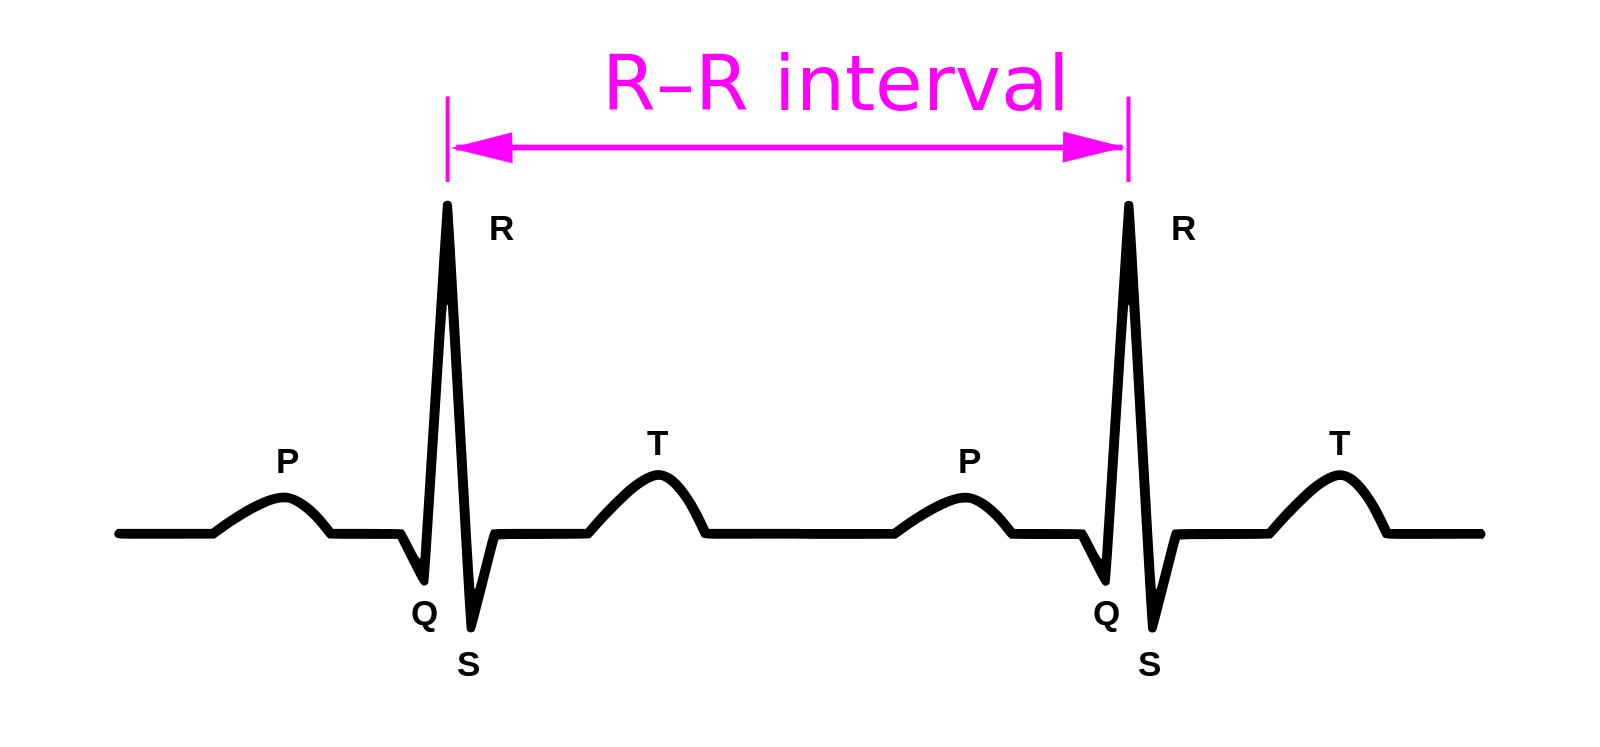
\includegraphics[width=1.0\textwidth]{img/RRInterval.png}
        	%\caption{RR Interval.}
        	\label{fig:rr}
        \end{figure}
        \textbf{Source:} \url{https://commons.wikimedia.org/wiki/File:ECG-RRinterval.svg}
    \end{frame}
    
    \begin{frame}{Introduction | Research Questions}
        \begin{itemize}
            \item Can you infer information about the patients age from RR Intervals?
            \item How can impurity been handled?
            \item Can RR Intervals be simulated?
        \end{itemize}
    \end{frame}
    
    \section{Related Literature}
    \begin{frame}{Related Literature}
        % Feature bases, presumably training only
        % Classification of trajectoriest
        % 60 healthy subjects, indicates inference is possible
        \begin{itemize}
            \item Patterns of Heart Rate Dynamics in Healthy Aging Population: Insights from Machine Learning Methods \cite{article}
            \item Classification of diffusion modes in single particle tracking data: feature based vs. deep learning approach \cite{unknown}
            \item Heart Rate Variability: Analysis and Classification of Healthy Subjects for Different Age Groups \cite{inproceedings}
        \end{itemize}
    \end{frame}
    
    \section{Data}
    \begin{frame}{Data | Data Sets}
        \begin{itemize}
            \item University of Gdansk
            \begin{itemize}
                \item 181 Holter recordings of 4 hours
                \item Sleep only
                \item Healthy patients
                \item Missing data points
            \end{itemize}
            \item PhysioNet: CAST RR Interval Sub-Study Database
            \begin{itemize}
                \item 1543 recordings of 24 hours
                \item Sleep and awake
                \item Survivors of myocardial infarction (heart attack)
                \item Treated with different medication
                \item No missing data points
            \end{itemize}
        \end{itemize}
    \end{frame}
    
    \begin{frame}{Data | Plots}
        \begin{figure}[hbt]
        	\center
        	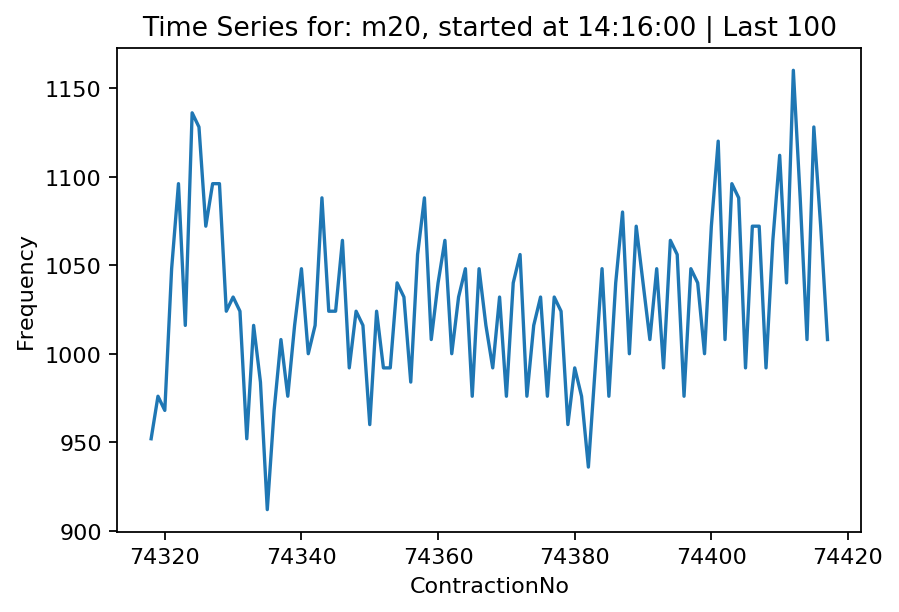
\includegraphics[width=1.0\textwidth]{img/example_data2.png}
        	%\caption{Example RR Intervals, 100 data points.}
        	\label{fig:example2}
        \end{figure}
    \end{frame}
    
    \begin{frame}{Data | Plots}
        \begin{figure}[hbt]
        	\center
        	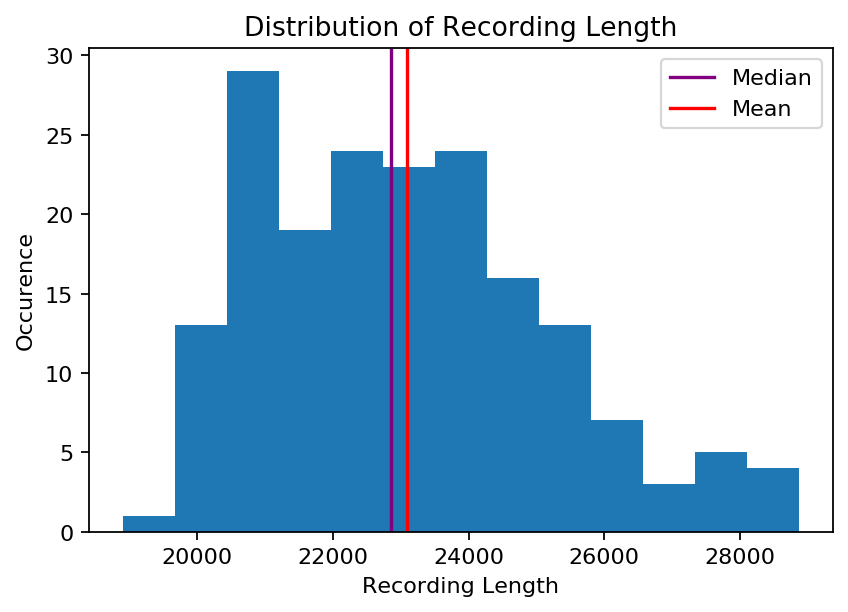
\includegraphics[width=1.0\textwidth]{img/record_length.png}
        	%\caption{RR Interval.}
        	\label{fig:record_length}
        \end{figure}
    \end{frame}
    
    \begin{frame}{Data | Plots}
        \begin{figure}[hbt]
        	\center
        	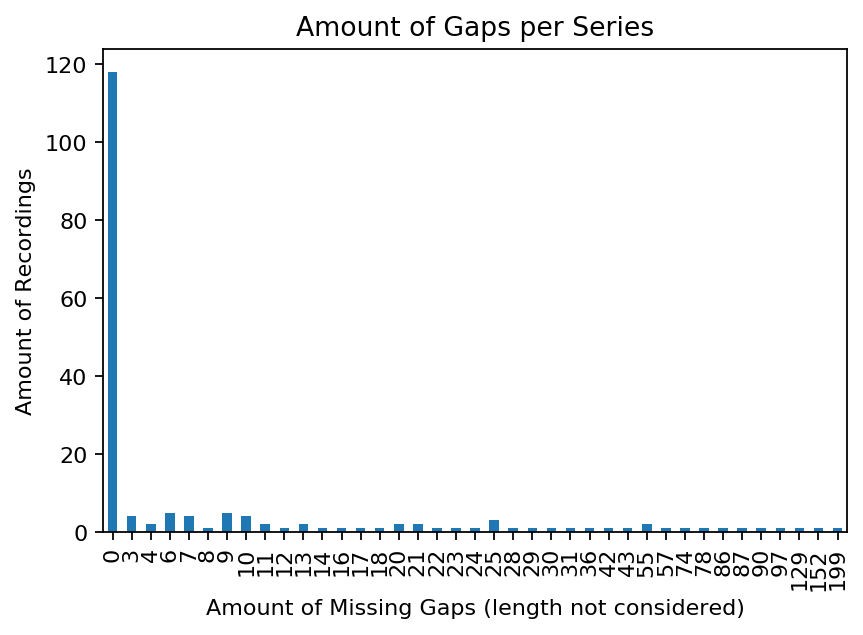
\includegraphics[width=1.0\textwidth]{img/gaps.png}
        	%\caption{RR Interval.}
        	\label{fig:gaps}
        \end{figure}
    \end{frame}
    
    \begin{frame}{Data | Plots}
        \begin{figure}[hbt]
        	\center
        	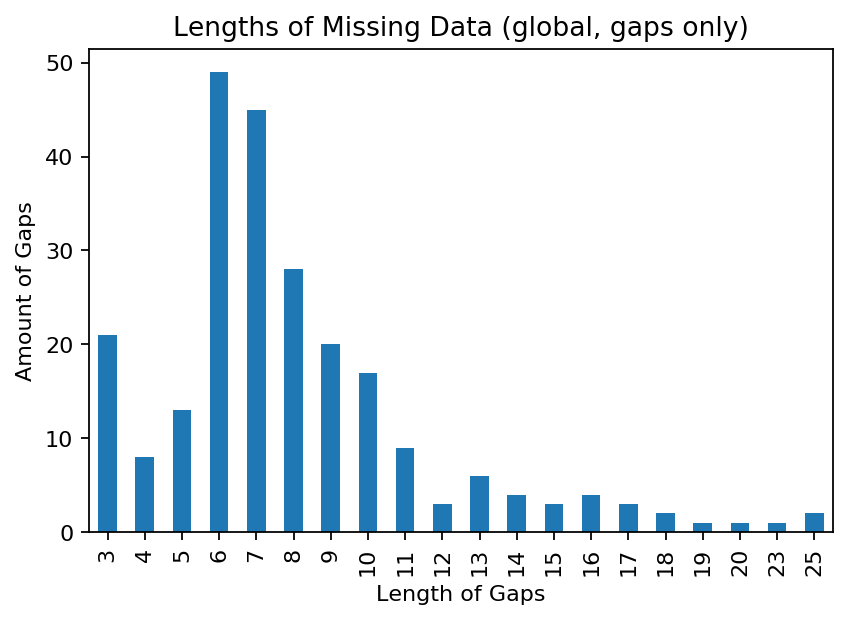
\includegraphics[width=1.0\textwidth]{img/length_missing_data.png}
        	\label{fig:length_missing_data}
        \end{figure}
    \end{frame}
    
    \section{Objectives}
    \begin{frame}{Objectives | Impurity}
        \begin{itemize}
            \item Splines
            \item Gaussian Processes (GPs)
        \end{itemize}
    \end{frame}
    
    \begin{frame}{Objectives | Impurity | Splines}
        \begin{figure}[hbt]
        	\center
        	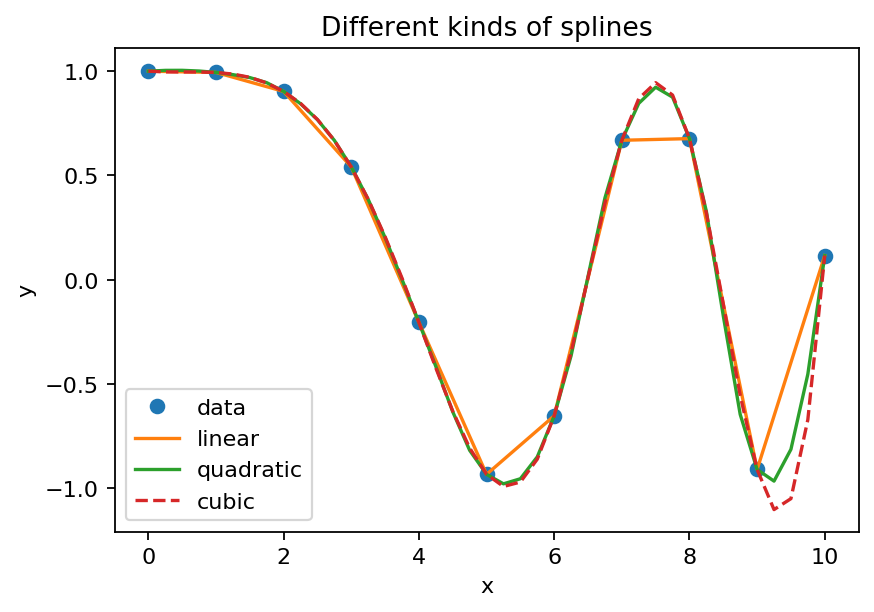
\includegraphics[width=1.0\textwidth]{img/splines.png}
        	\label{fig:splines}
        \end{figure}
    \end{frame}
    
    \begin{frame}{Objectives | Impurity | GPs}
        \begin{figure}[hbt]
        	\center
        	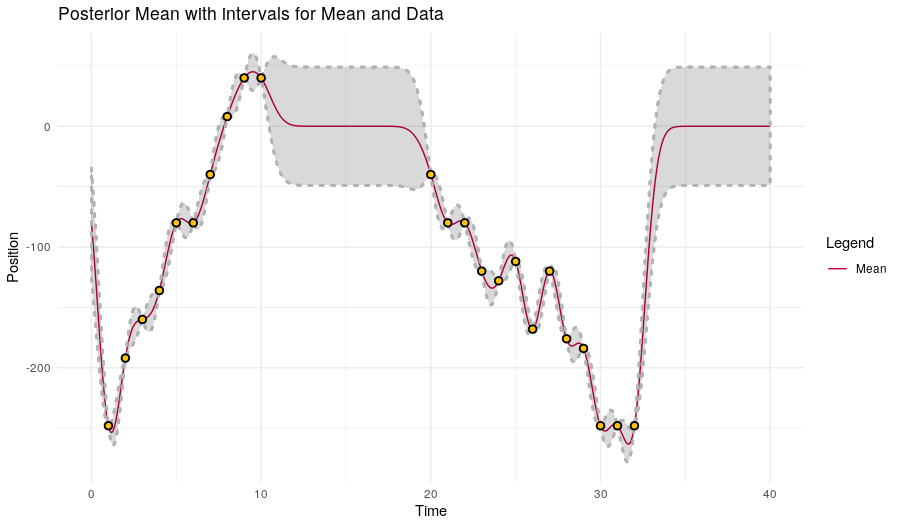
\includegraphics[width=1.0\textwidth]{img/gp.png}
        	\label{fig:gp}
        \end{figure}
    \end{frame}
    
     \begin{frame}{Objectives | Classification}
        \begin{itemize}
            \item Feature based Machine Learning Methods*
            \item Deep Learning - Convolutional Neural Networks (CNNs)
        \end{itemize}
    \end{frame}
    
    \begin{frame}{Objectives | Simulation | GP}
        Sampling from the Posterior of the GP
        \begin{itemize}
            \item $f(x) \sim \mathcal{GP} (m(x), k(x, x'))$
            \item $m(x)$ is the mean function, $k(x, x')$ the kernel function
            \item $K_{OU}(x, x') = \text{exp} \Big(- \frac{|d|}{\ell} \Big)$
            \item $K_{LP} = \sigma^2 \text{exp} \Big( - \frac{2}{\ell^2} \text{sin} \Big( \pi \frac{|x - x'|}{p} \Big) \Big) \text{exp} \Big( - \frac{(x - x')^2}{2\ell^2} \Big)$
            \label{fig:local_periodic_kernel}
        \end{itemize}
    \end{frame}
    
    \begin{frame}{Objectives | Simulation | GP}
        \center
    	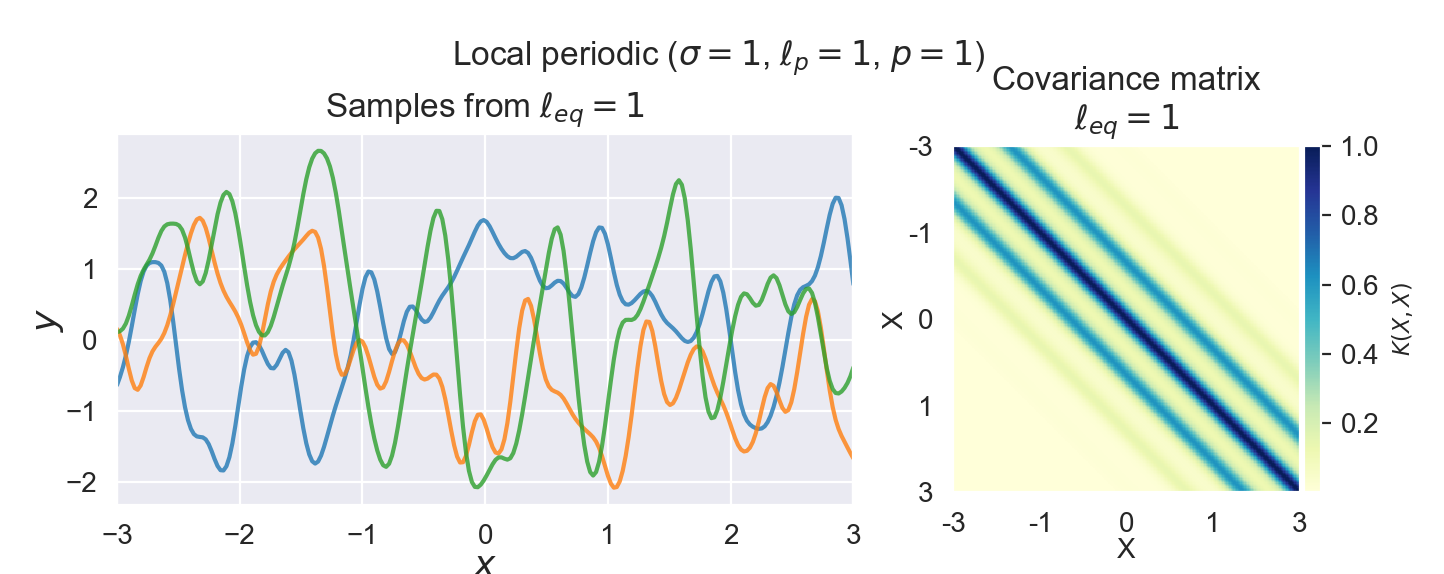
\includegraphics[width=1.0\textwidth]{img/local_periodic_kernel.png}
    	\textbf{Source:} \url{https://peterroelants.github.io/posts/gaussian-process-kernels/}
    \end{frame}
    
    \begin{frame}{Objectives | Simulation | OU}
        Fitting an Ornstein–Uhlenbeck (OU) process
        \begin{itemize}
            \item Stochastic Differential Equation (SDE)
            \item $dx_t = \theta (\mu - x_t)d_t + \sigma d W_t$
            \item $\mu$ is the long-term mean
            \item $\theta$ defines the speed of mean reversion
            \item $\sigma$ defines the randomness
            \item $W_t$ is the \textit{Wiener process}
            \item $\Rightarrow$ Using a trigonometric function as the optimum function
        \end{itemize}
    \end{frame}
    
    \begin{frame}{Objectives | Simulation | OU}
        \begin{figure}[hbt]
        	\center
        	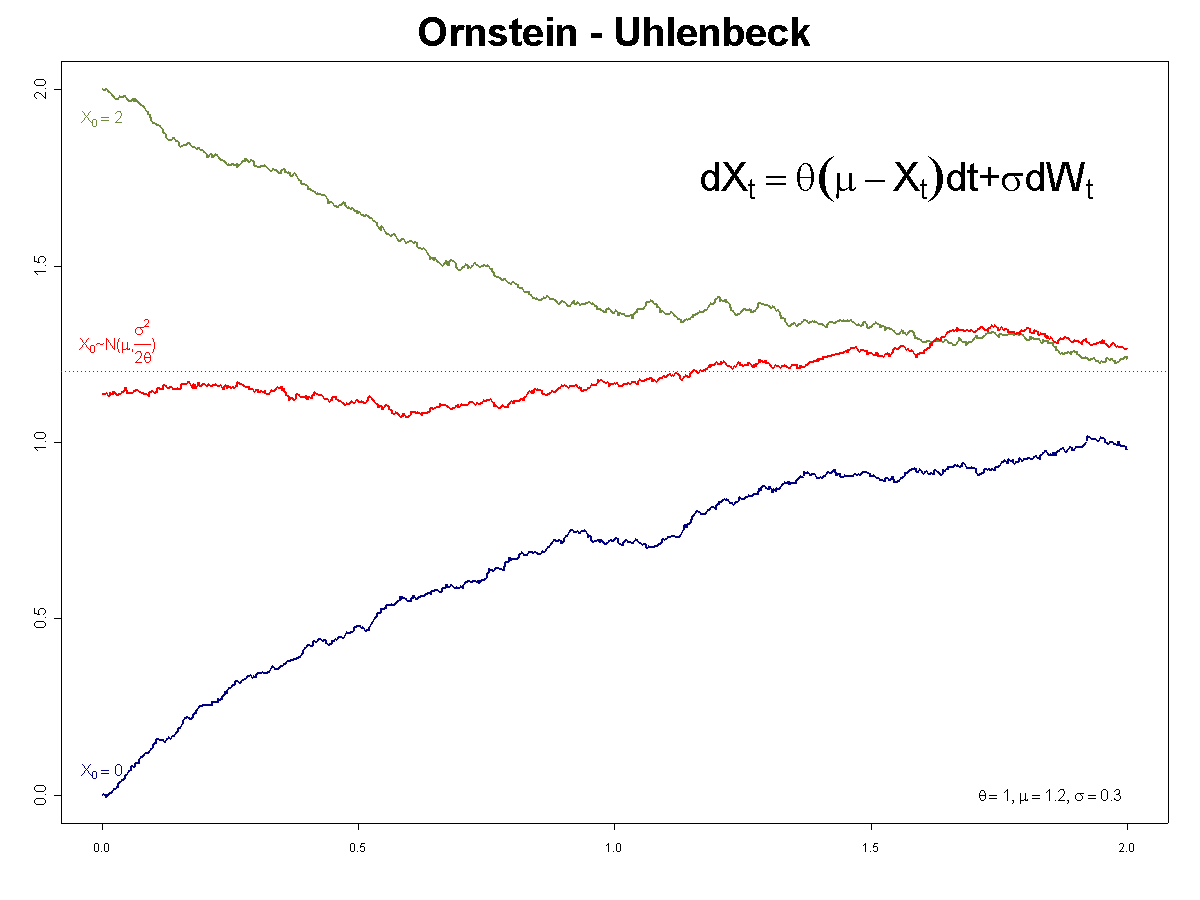
\includegraphics[width=0.9\textwidth]{img/ou_process.png}
        	%\caption{Lengths of missing data.}
        	\label{fig:ou_process}
        \end{figure}
    \end{frame}
    
    
    \section{Status and Outlook}
    \begin{frame}{Status and Outlook}
        \begin{itemize}
            \item Impurity
                \begin{itemize}
                    \item (done) Splines (linear, quadratic, cubic)
                    \item (open) GP, possibly in TensorFlow Probability (TFP), \textbf{very large} covariance matrix
                \end{itemize}
            \item Classification
                \begin{itemize}
                    \item (done) Simply CNN yields in very bad results
                    \item (open) More advanced CNN, maybe combine with Recurrent Neural Networks (RNNs)
                    \item Utilise Long Short-Term Memory Cells (LSTMs)
                \end{itemize}
            \item Simulation
                \begin{itemize}
                    \item (open) Sampling from GP
                    \item (open) Fitting OU process
                \end{itemize}
            \item Evaluation
        \end{itemize}
    \end{frame}
    
    \appendix
    
    \begin{frame}[standout]{}
        \center Appendix
    \end{frame}
    
    \begin{frame}{Objectives | Classification | CNN}
        \begin{figure}[hbt]
        	\center
        	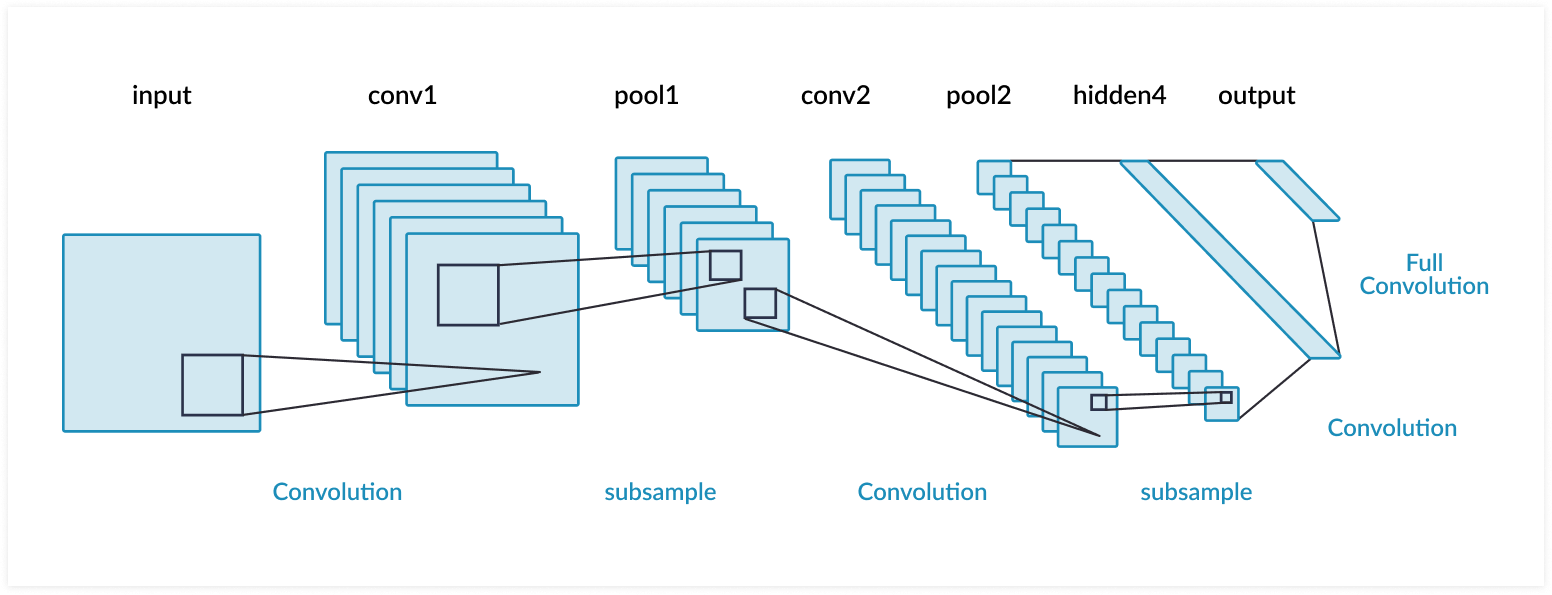
\includegraphics[width=1.0\textwidth]{img/cnn_example.png}
        	\label{fig:cnn_example}
        \end{figure}
    \end{frame}
    
    \begin{frame}{Objectives | Classification | CNN}
        \begin{figure}[hbt]
        	\center
        	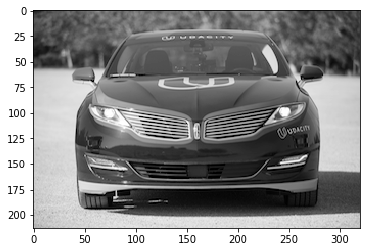
\includegraphics[width=0.5\textwidth]{img/car.png}
        	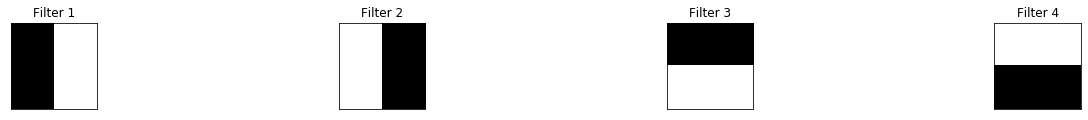
\includegraphics[width=1.0\textwidth]{img/filters_pure.png}
        	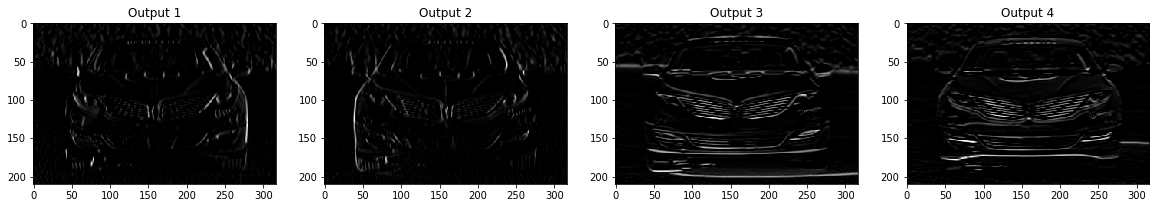
\includegraphics[width=1.0\textwidth]{img/filters.png}
        	\label{fig:filters}
        \end{figure}
    \end{frame}
    
    \begin{frame}[allowframebreaks]{References}
    
      \bibliography{literature.bib}
      \bibliographystyle{apalike}
    
    \end{frame}
    
\end{document}